\subsection{Implementation architecture}
The implementation of the algorithm was developed using the Python programming language which allows work quickly and integrate systems more effectively.
As data persistence, a MySql relational database was used. All of the above was mounted on an instance of the free Amazon layer, specifically EC2 - Linux.
%------------------------
As a source code control system, GIT was used, which allowed to maintain a control of local source code for both the developed algorithm and the documentation associated to this thesis. Constant replicas were performed against a GIT cloud repository, specifically GITHUB.
 
\subsection{Binary Global-Best Harmony Search Metaheuristic}
The parameters presented below were the result of exhaustive tests and multiple executions that allowed to test beyond the random components a correct behavior for metaheuristics, that is to say, presenting a higher degree of effectiveness compared to other metaheuristics.

The process begins with the generation of an initial population of harmonies that are vectors composed of binary digits $d$, in a repetition of the process that is called improvisation. The number of improvisations is denoted by $NI$. Once the improvisations are finished, there are a number of harmonies on which a repair process is executed with two-phase repair operator (Algorithm \ref{alg:addAndDrop}). Once the harmonies are repaired and meet the constraints defined in the  Matrix $A$ for the SCP, the best and worst harmony, denoted by $x_ {best}$ and $x_ {worst}$, respectively, are stored. The detail of the behavior of the metaheuristics can be reviewed in the flow chart (Figure \ref{dia:FlowBGBHS}). Additionally a greedy selection mechanism are integrated into the BGBHS. The greedy operation is based on the idea that the item with higher profit density ratio should be used first. And the profit density ratio can be calculated by the equation (\ref{ec:mu_j}): 

\begin{equation} \label{ec:mu_j} 
\mu_{j}={\frac{1}{c_j}}
\end{equation}	
		

%------------------------------Diagrama de HS
\begin{figure}[]
\centering
\begin{tikzpicture}[align = flush center, font = \small, node distance = 12mm, scale=0.6, every node/.style={scale=0.6}] %[node distance = 15mm, auto]
\node (start) [startstop] {Start};
\node (pro1) [process, below of=start] {Initialize parameters};
\node (pro2) [process, below of=pro1] {Initialize Harmony Memory (HM)};
\node (pro3) [process, below of=pro2] {Repair all harmonies in HM};
\node (pro4) [process, below of=pro3] {$t=1$};
\node (pro5) [process, below of=pro4] {Save $x_{best}$ and $x_{worst}$ harmony};
\node (proB) [process, below of=pro5]{$x_{new} = $ Bernoulli trial \smallskip $\forall {x_{new}}_j \in \{0,1\}$, and $j=\{1 \dots n\}$};
\node (pro6) [process, below of=proB] {Rand() $\leq$ HMCR};
\node (pro7) [process, below of=pro6] {Rand() $\leq$ PAR};
\node (pro8) [decision, below of=pro7] {$j < n$};
\node (pro9) [process, left of=pro8, xshift=-1.5cm] {$j = j + 1$};
\node (pro10) [decision, below of=pro8, yshift=-0.2cm] {$x_{new}$ is better than $x_{best}$};
\node (pro11) [process, right of=pro10, xshift=4.0cm] {$x_{best} = x_{new}$};
\node (pro12) [decision, below of=pro10, yshift=-1.0cm] {$x_{new}$ is better than $x_{worst}$};
\node (pro13) [process, right of=pro12, xshift=2.5cm] {$x_{worst} = x_{new}$};
\node (pro14) [decision, below of=pro12, yshift=-1.0cm] {Termination criterion is met?};
\node (pro15) [process, left of=pro14, xshift=-3.5cm] {$t=t+1$};
\node (pro16) [process, below of=pro14, yshift=-0.8cm] {Output Result};

%---------------------------------ARROWS
\draw [arrow] (start) -- (pro1);
\draw [arrow] (pro1) -- (pro2);
\draw [arrow] (pro2) -- (pro3);
\draw [arrow] (pro3) -- (pro4);
\draw [arrow] (pro4) -- (pro5);
\draw [arrow] (pro5) -- (proB);
\draw [arrow] (proB) -- (pro6);
\draw [arrow] (pro6) -- (pro7);
\draw [arrow] (pro7) -- (pro8);
\draw [arrow] (pro8) -- (pro9) node [midway, above] {Y};
\draw [arrow] (pro9) |- (pro6);
\draw [arrow] (pro8) -- (pro10) node [midway, left] {N};
\draw [arrow] (pro10) -- (pro11) node [midway, above] {Y};
\draw [arrow] (pro10) -- (pro12) node [midway, left] {N};
\draw [arrow] (pro12) -- (pro13) node [midway, above] {Y};
\draw [arrow] (pro12) -- (pro14) node [midway, left] {N};
\draw [arrow] (pro14) -- (pro15) node [midway, above] {N};
\draw [arrow] (pro15) |- (pro5);
\draw [arrow] (pro11) |- (pro14) ;
\draw [arrow] (pro13) |- (pro14) ;
\draw [arrow] (pro14) -- (pro16) ;

\end{tikzpicture}
\caption{Flowchart of BGBHS algorithm.}\label{dia:FlowBGBHS}
\end{figure}
%------------------------------END Diagrama de HS

The HS is good at identifying the high performance regions of the solution space in a reasonable time, but poor at performing local search \cite{DBLP:journals/eswa/XiangALHZ14}. Namely, there is an unbalance between the exploration and the exploitation of HS. 
 
To solve the problem of local exploitation, we propose a variable parameter for the Bernoulli probability $p$, which starts from one and decreases with each iteration, tending to zero (Figure \ref{fig:pvalue}). This will allow solutions in a first instance to have more variables activated and as the iterations pass, the probability that a variable is activated will be closed to zero.
 

\begin{figure}[]
\centering
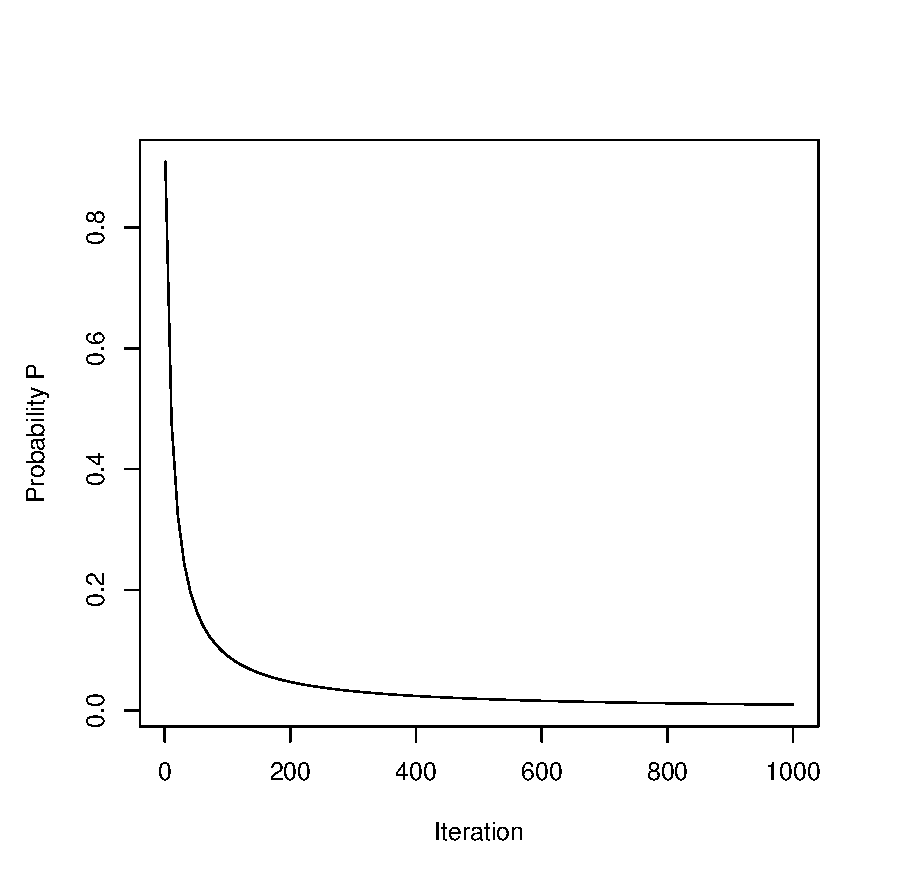
\includegraphics[scale=.45]{Implementacion/img/p_bernoulli.eps}
\caption{$p$ value over iteration}
\label{fig:pvalue}
\end{figure}


The initial population in BGBHS is generated randomly using a Bernoulli process. In probability and statistics, a Bernoulli process is a finite or infinite sequence of binary random variables, so it is a discrete-time stochastic process that takes only two values $\{1,0\}$, success (equation \ref{ec:bernoullie_p}) or failure (equation \ref{ec:bernoullie_p-1}), given the probability $p$. A Bernoulli process is a finite or infinite sequence of independent random variables $x_1$, $x_2$, $x_3$,\dots,$x_n$  $\forall x \in \{0,1\}$ ~ and ~ $i=\{1,\dots, n\}$.

\begin{equation} \label{ec:bernoullie_p} 
P(x_i=1) = P(\text{success at the $i$-th trial}) = p 
\end{equation}	

\begin{equation} \label{ec:bernoullie_p-1} 
P(x_i=0) = P(\text{failure at the $i$-th trial}) = 1-p
\end{equation}	

Specifically, for each decision variable of an initial harmony vector, a number within is generated randomly. If the value of the number is less than $p$, the corresponding variable takes 0; otherwise it takes 1. In this way, a set of HMS harmonies will be generated randomly.


%------------------------------Fase ADD y DROP:
\begin{algorithm}
\begin{algorithmic}[1]
 \STATE //ADD Phase
\STATE $M \gets 1,2,\ldots, m$
\STATE $A_i \sum_{j=1}^{n} a_{ij}x_{j}, i \in M$
\FOR{$j \gets 1$ \TO $n$} {
	\IF{$x_j = 0$ and $\exists i \in M, A_i < 1$ } {
		\STATE $x_j \gets 1$
		\STATE $A_i \gets A_i + a_{ij}$
	}\ENDIF
} \ENDFOR

\STATE //DROP Phase
\FOR{$j \gets n$ \TO $1$}{
	\IF{$x_j = 1$ and $\exists i \in M, A_i - a_{ij} \geq 1$ } {
		\STATE $x_j \gets 0$
		\STATE $A_i \gets A_i - a_{ij}$
	}\ENDIF
} \ENDFOR

\caption{Repair operator ADD and DROP}\label{alg:addAndDrop}
\end{algorithmic}
\end{algorithm}


%------------------------------nueva_armonia_agresiva():

